%\documentclass[handout]{beamer}
\documentclass[10pt]{beamer}
\usetheme[
  outer/progressbar=foot,
  outer/numbering=none
]{metropolis}
\usepackage{amsmath, amssymb, amsthm, mathtools,media9}
\usepackage[export]{adjustbox}

\usepackage[default]{sourcesanspro}
\usepackage[utf8]{inputenc}
\usepackage[T1]{fontenc}
\metroset{titleformat=smallcaps}

\usepackage{tikz}
\usetikzlibrary{mindmap,shadows}
\usepackage{animate}
\usepackage[compatibility=false]{caption}

\usepackage{subcaption}
\usepackage{graphicx}
\usetikzlibrary{spy,calc,patterns,arrows,decorations.pathmorphing,backgrounds,positioning,fit,petri,mindmap,trees,intersections}
\usepackage{graphicx}
\usepackage{keystroke}
\usepackage{color}
\usepackage{multicol}
%\usepackage{multimedia}
\usepackage{enumerate}
\usepackage{multirow}
\usepackage{pgfplots,tikz,tcolorbox}
\usepackage{appendixnumberbeamer}



\pgfplotsset{compat=newest}
%\expandafter\def\expandafter\insertshorttitle\expandafter{%
 % \insertshorttitle\hfill\insertframenumber\,/\,\inserttotalframenumber}
%\usepackage{enumitem}


%\usepackage[T1]{fontenc}
\usepackage{color,hyperref}
\definecolor{darkblue}{rgb}{0.0,0.0,0.5}
%\hypersetup{colorlinks,breaklinks,
%            linkcolor=darkblue,urlcolor=darkblue,
%            anchorcolor=darkblue,citecolor=darkblue}
\usetikzlibrary{patterns}
\usetikzlibrary{decorations.pathmorphing,backgrounds,positioning,fit,petri,mindmap,trees}
\usepgflibrary{arrows,shapes.geometric}
\usepgflibrary{shapes.symbols}
%\hypersetup{colorlinks,breaklinks,linkcolor=darkblue,urlcolor=darkblue,anchorcolor=darkblue,citecolor=darkblue}
\usetikzlibrary{spy,calc,patterns,arrows,decorations.pathmorphing,backgrounds,positioning,fit,petri,mindmap,trees,intersections}
\usepackage{color}
\usepackage{multirow}
\usetikzlibrary{arrows,positioning} 
\tikzset{
    %Define standard arrow tip
    >=stealth',
    %Define style for boxes
    punkt/.style={
           rectangle,
           rounded corners,
           draw=black, very thick,
           text width=8.5em,
           minimum height=2em,
           text centered},
    % Define arrow style
    pil/.style={
           ->,
           thick,
           shorten <=2pt,
           shorten >=2pt,}
}


\usepackage{listings}




%\usepackage[hang]{footmisc}
%\setlength\footnotemargin{10pt}

\setbeamertemplate{caption}[numbered]
\usepgfplotslibrary{statistics}

\usetikzlibrary{fadings}
\tikzfading[name=fade out,
  inner color=transparent!0, outer color=transparent!100]

%\setbeameroption{show notes}

\newcommand\xqed[1]{%
  \leavevmode\unskip\penalty9999 \hbox{}\nobreak\hfill
  \quad\hbox{#1}}
\newcommand\eqed{\xqed{$\blacktriangle$}}

\title{Generalized Extreme Value Distribution}
\subtitle{}
%\institute{SUTD}
\author{Zhangsheng Lai}
\date{\today}

\newcommand{\sol}{\textbf{Solution\\}}
\pgfmathdeclarefunction{gauss}{2}{%
  \pgfmathparse{1/(#2*sqrt(2*pi))*exp(-((x-#1)^2)/(2*#2^2))}%
}
%\pgfmathdeclarefunction{gauss1}{2}{%
  %\pgfmathparse{(1/(#2*sqrt(2*pi))*exp(-((-x-#1)^2)/(2*#2^2)))*exp(-x)}%
%}
\pgfmathdeclarefunction{gauss2}{2}{%
  \pgfmathparse{(1/(#2*sqrt(2*pi))*exp(-0.5*abs(x)-#1)*(sqrt(abs(x)))}%
}

%\pgfmathdeclarefunction{gauss2}{2}{%
  %\pgfmathparse{(1/(#2*sqrt(2*pi))*exp(-((x-#1)^2)/(2*#2^2)))*exp(x)}%
%}
\pgfmathdeclarefunction{gauss1}{2}{%
  \pgfmathparse{(1/(#2*sqrt(2*pi))*exp(-0.5*x-#1)*(sqrt(x))}%
}
\def\checkmark{\tikz\fill[scale=0.4](0,.35) -- (.25,0) -- (1,.7) -- (.25,.15) -- cycle;}

\newcommand*{\Perm}[2]{{}^{#1}\!P_{#2}}%
\newcommand*{\Comb}[2]{{}^{#1}C_{#2}}%
\begin{document}


\begin{frame}
\titlepage
\end{frame}


%\begin{frame}
%\tableofcontents
%\end{frame}

\begin{frame}{Motivation}
\begin{alertblock}{Prediction of Extremal Precipitation}
For the 10th Extreme Value Analysis Conference, they proposed a challenge to predict spatio-temporal extremes. Training data consisting of 30 years of rainfall from 40 weather stations around Paris are given for contestants to predict the extreme monthly precipitation over the next 20 years. On the daily range, this event corresponds to a quantile level 
\begin{align*}
0.998 = 1 - 0.002 \approx 1- \frac{1}{20 \times 30 \text{days}}
\end{align*}
\end{alertblock}
\end{frame}

\begin{frame}{Model Formulation}
The model focuses on the statistical behaviour of $M_n = \max\{X_1,\ldots,X_n\}$ where all the $X_i$'s are independent and identically distributed with distribution function $F$. The distribution of $M_n$ can be derived exactly for all values of $n$
\begin{align}
\mathbb{P}\{M_n\leq z\} &= \mathbb{P}\{X_1\leq z , \ldots X_n \leq z\}\nonumber\\
&= \prod_{i=1}^{n}\mathbb{P}\{X_i\leq z\}\nonumber\\
&=\{F(z)\}^n \label{eq:maxofrv}
\end{align}
\end{frame}


%\begin{frame}{Model Formulation}
%Although we know how to find the distribution of $M_n$ the maximum of independent and identically distributed random variables, not knowing what $F$ makes knowing the above not helpful. We could utilise standard statistical techniques like maximum likelihood to get an estimate $\widehat{F}$ from the observed data the substitute into (\ref{eq:maxofrv}). However small errors in the estimate of $F$ can lead to substantial errors in $F^n$.
%
%The approach we are going to look at here is to accept that $F$ is unknown, instead of estimating $F$ to estimate $F^n$, we find an estimate of $F^n$ directly, which can be estimated using extreme data only. The idea is similar to the usual method of approximating the distribution of sample means by the normal distribution. So essentially we are doing the extreme value analogue of the central limit theory.
%\end{frame}

\begin{frame}{Model Formulation}
Problems encountered:
\begin{itemize}
\item not knowing what $F$ is does not allow us to find the distribution of $M_n$.
\item maximum likelihood can be used to get an estimate $\widehat{F}$, but small errors in the estimate of $F$ can lead to substantial errors in $F^n$.
\end{itemize}
The approach to the problem is to find an estimate of $F^n$ directly using extreme data only which gives us the extreme value analogue of the central limit theory.
\end{frame}

\begin{frame}{Model Formulation}
Observe that for a distribution function $F$ with upper end-point $z^+$, i.e. $z^+$ is the smallest value of $z$ such that $F(z^+) = 1$, for any $z<z^+, F^n(z) \to 0$ as $n \to \infty$, thus $M_n$ degenerates to a point mass on $z^+$. 

To avoid this problem, we do a linear renormalization of the variable $M_n$:
\begin{align*}
M_n^\ast = \frac{M_n - b_n}{a_n}
\end{align*}
for a sequence of constants $\{a_n>0\}$ and $\{b_n\}$. By choosing appropriate $\{a_n\}$ and $\{b_n\}$ it stabilizes the location and scale of $M_n^\ast$ as $n$ grows avoiding problems of degeneracy. %Thus we seek limit distributions of $M_n^\ast$ instead of $M_n$ with appropriate choices of $\{a_n\}$ and $\{b_n\}$.

\end{frame}

\begin{frame}{Extremal Types Theorem}
\begin{theorem}[Fisher-Tippett-Gnedenko]\label{thm:gfw}
If there exists sequences of constants $\{a_n>0\}$ and $\{b_n\}$ such that 
\begin{align*}
\mathbb{P}\{(M_n-b_n)/a_n \leq z\} \to G(z) \quad \text{ as } n \to \infty
\end{align*}
where $G$ is a non-degenerate distribution function, then $G$ belongs to one of the following families:
\begin{align*}
\text{Gumbel}:\quad G(z)\quad&= \quad\exp \left\{-\exp\left[-\left(\frac{z-b}{a}\right)\right]\right\}, \quad -\infty<z<\infty\\
\text{Fr\'echet}: \quad G(z)\quad&= \quad\begin{cases}
0, & z \leq b\\
\exp\left\{-\left(\frac{z-b}{a}\right)^{-\alpha}\right\}, &z >b
\end{cases}
\\
%\mathbb{III}:\quad G(z)\quad&=  \quad\begin{cases}
%\exp\left\{-\left[-\left(\frac{z-b}{a}\right)^{-\alpha}\right]\right\}, & z \leq b\\
%1, &z >b
\text{Weibull}:\quad G(z)\quad&=  \quad\begin{cases}
\exp\left\{-\left(-\frac{z-b}{a}\right)^{\alpha}\right\}, & z \leq b\\
1, &z >b
\end{cases}
\end{align*}
for parameters $a>0, b$ and for families Fr\'echet and Weibull, $\alpha >0$.
\end{theorem}
\end{frame}


%\begin{frame}{Extremal Types Theorem}
%These three classes of distribution are called \textbf{extreme value distributions} with the types $\mathbb{I},\mathbb{II}$ and $\mathbb{III}$ widely known as the \textbf{Gumbel}, \textbf{Fr\'echet} and \textbf{Weibull} families respectively. Theorem \ref{thm:gfw} implies that when $M_n$ can be stabilized with suitable sequences $\{a_n>0\}$ and $b_n$ the corresponding normalized $M_n^\ast$ has a limiting distribution that must be one of the three extreme distributions. It is in this sense that the theorem provides an extreme value analog of central limit theorem.
%\end{frame}

\begin{frame}{Extremal Types Theorem}
A much more flexible approach is to reformulate the three models into a single distribution which has the form,
\begin{align}\label{eq:gev}
G(z) = \exp \left\{-\left[1+\xi\left(\frac{z-\mu}{\sigma}\right)\right]^{-1/\xi}\right\}
\end{align}
defined on the set $\{z : 1 + \xi(z-\mu)/\sigma>0\}$ where the parameters satisfy $-\infty<\mu, \xi<\infty$ and $\sigma >0$. The $\mu$ is the location parameter, $\sigma$ is the scale parameter and $\xi$ is the shape parameter.

%The above distribution is the generalized extreme value (GEV) family of distributions, where $\mu$ is the location parameter, $\sigma$ is the scale parameter and $\xi$ is the shape parameter. The Fr\'echet and Weibull classes correspond to the case where $\xi >0$ and $\xi<0$ respectively and the subset of the family with $\xi = 0$ is interpreted as the limit of (\ref{eq:gev}) as $\xi \to 0$.
\end{frame}

\begin{frame}{Extremal Types Theorem}
\begin{theorem}[Generalized Extreme Value]\label{thm:gev}
If there exists sequence of constants $\{a_n>0\}$ and $\{b_n\}$ such that 
\begin{align}\label{eq:gevlimit}
\mathbb{P}\{(M_n - b_n)/a_n\leq z\} \to G(z) \quad\text{ as } n \to \infty
\end{align}
for a non-degenerate distribution function $G$, then $G$ is a member of the GEV family
\begin{align}
G(x) = \exp \left\{-\left[1+\xi\left(\frac{x-\mu}{\sigma}\right)\right]^{-1/\xi}\right\}
\end{align}
defined on the set $\{x : 1 + \xi(x-\mu)/\sigma>0\}$ where the parameters satisfy $-\infty<\mu, \xi<\infty$ and $\sigma >0$.
\end{theorem}
\end{frame}

\begin{frame}{Extremal Types Theorem}
By interpreting the limit in Theorem \ref{thm:gev} as an approximation for large values of $n$, suggests the use of the GEV family for modelling the distribution of maxima of long sequences. %With this result we can solve for the normalizing constants that are unknown in practice. 
Given (\ref{eq:gevlimit}) holds
\begin{align*}
\mathbb{P}\{(M_n-b_n)/a_n\leq z\} \approx G(z)
\end{align*}
for large $n$. Equivalently,
\begin{align*}
\mathbb{P}\{M_n\leq z\} \approx G((z-b_n)/a_n) = G^\ast(z)
\end{align*}
where $G^\ast$ is another member of the GEV family. This says that if we can approximate the distribution of $M_n^\ast$ by a member of the GEV for large $n$, the distribution of $M_n$ itself can also be approximated by a different member of the same family.
\end{frame}

\begin{frame}{Outline Proof of the Extremal Types Theorem}
\begin{definition}
A distribution $G$ is said to be \emph{max-stable} if, for every $n=2,3,\ldots$ there are constants $\alpha_n>0$ and $\beta_n$ such that
\begin{align*}
G^n(\alpha_nz+\beta_n) = G(z)
\end{align*}
\end{definition}
\end{frame}

\begin{frame}{Outline Proof of the Extremal Types Theorem}
\begin{theorem}\label{thm:maxstablegev}
A distribution is max-stable iff it is a generalized extreme value distribution.
\begin{proof}
We shall skip the forward direction proof as it is very involved. To show the converse, let the Fr\'echet $G(x)$ be given, then choosing $\alpha_n = n^{1/\alpha}$ and $\beta_n = b(1-n^{1/\alpha})$
\begin{align*}
G^n(z\alpha_n+\beta_n) &= \exp\left\{-n\left(\frac{zn^{1/\alpha}+b(1-n^{1/\alpha})-b}{a}\right)^{-\alpha}\right\}\\
&= \exp\left\{-n\left(\frac{zn^{1/\alpha}-bn^{1/\alpha}}{a}\right)^{-\alpha}\right\}\\
&= \exp\left\{-\left(\frac{z-b}{a}\right)^{-\alpha}\right\}=G(z)
%&=G(n^{-1/\alpha}z+(1 +  n^{-1/\alpha}))
\end{align*}
In a similar fashion we can prove it for Weibull. 
\end{proof}
\end{theorem}
\end{frame}

\begin{frame}{Outline Proof of the Extremal Types Theorem}
\begin{proof}
For Gumbel, choose $\alpha_n = 1$ and $\beta_n = a\log n$, 
\begin{align*}
G^n(z\alpha_n+\beta_n) &= \exp\left\{-n\exp\left[-\left(\frac{z+a\log n-b}{a}\right)\right]\right\} \\
&= \exp\left\{-n\exp\left[-\left(\frac{z-b}{a}\right)-\log n\right]\right\} \\
%G^n(z) &= \exp\left\{-n\exp\left[-\left(\frac{z-b}{a}\right)\right]\right\} \\
&= \exp\left\{-n\cdot n^{-1}\exp\left[-\left(\frac{z-b}{a}\right)\right]\right\}\\
&= \exp\left\{-\exp\left[-\left(\frac{z-b}{a}\right)\right]\right\} \\
&=G(z)
\end{align*}
%where $\alpha_n = 1$ and $\beta_n = -a\log n$.
\end{proof}
\end{frame}

\begin{frame}{Outline Proof of the Extremal Types Theorem}
Theorem \ref{thm:maxstablegev} is used directly in the proof of extremal types theorems. We start be considering $M_{nk}$, the maximum random variable in a sequence of $n \times k$ variables for some large value of $n$. This can be regarded as the maximum of a single sequence of length $n \times k$ or as the maximum of $k$ maxima, each of which is a maximum of $n$ observations. Let's assume that the limit distribution of $(M_n-b_n)/a_n$ is $G$, thus for sufficiently large $n$
\begin{align*}
\mathbb{P}\{(M_n-b_n)/a_n\} \approx G(z)
\end{align*}
\end{frame}

\begin{frame}{Outline Proof of the Extremal Types Theorem}
Hence for any integer $k$ we also have 
\begin{align*}
\mathbb{P}\{(M_{nk}-b_{nk})/a_{nk}\} \approx G(z)
\end{align*}
but now we recall the definitions of $M_n$ and $M_{nk}$, we have 
\begin{align*}
\mathbb{P}\{(M_{nk}-b_{nk})/a_{nk}\leq z\}=\left[\mathbb{P}\{(M_{n}-b_{n})/a_{n}\leq z\}\right]^k
\end{align*}
using the equations above,
\begin{align*}
\mathbb{P}\{M_{nk}\leq z\} &\approx G\left(\frac{z-b_{nk}}{a_{nk}}\right)\\
\text{ and }\quad\mathbb{P}\{M_{nk}\leq z\} &\approx G^k\left(\frac{z-b_{n}}{a_{n}}\right)
\end{align*}

%\begin{align*}
%G\left(\frac{z-b_{nk}}{a_{nk}}\right)&\approx\mathbb{P}\{(M_{nk}-b_{nk})/a_{nk}\leq z\}\\
%&=\left[\mathbb{P}\{(M_{n}-b_{n})/a_{n}\leq z\}\right]^k \approx G^k\left(\frac{z-b_n}{a_n}\right)
%\end{align*}
Therefore $G$ and $G^k$ are identically apart except for location and scale coefficients. Thus $G$ is max-stable and a member of GEV by Theorem \ref{thm:maxstablegev}
\end{frame}

\begin{frame}{Example}
\begin{example}
If $X_1, X_2, \ldots$ is a sequence of independent and identically distributed $\text{\sffamily Exp}(1)$ random variables, $F(x) = 1-e^{-x}$ for $x>0$, choosing $a_n = 1$ and $b_n = \log n$
\begin{align*}
\mathbb{P}\{(M_n-b_n)/a_n\leq z\} &= F^n(z + \log n)\\
&= \bigg[1-e^{-(z+\log n)}\bigg]^n\\
&= \bigg[1-n^{-1}e^{-z}\bigg]^n \to \exp(-e^{-z}) \text{ as } n \to \infty
\end{align*}
here we use the fact that $\lim_{n \to \infty} \left(1-\frac{1}{n}\right)^n = \frac{1}{e}$. Hence with the chosen $a_n$ and $b_n$, the limit of $M_n$ converges to the Gumbel distribution as $n \to \infty$. This corresponds to $\xi = 0$ in the GEV family. \eqed
\end{example}
\end{frame}




\begin{frame}{Example}
\begin{example}
If $X_1, X_2, \ldots$ is a sequence of independent Fr\'echet variables, $F(x) = \exp(-1/x)$ for $x>0$. Letting $a_n = n$ and $b_n = 0$
\begin{align*}
\mathbb{P}\{(M_n-b_n)/a_n\leq z\}  & = F^n(nz)\\
& = \Big[\exp\{-1/nz\}\Big]^n\\
& = \exp(-1/z)
\end{align*}
as $n \to \infty$, for each $z>0$. Hence the limit in this case which is an exact result for all $n$ since the Fr\'echet is max-stable is also the Fr\'echet distribution. This corresponds to $\xi = 1$ in the GEV family.
\eqed
\end{example}
\end{frame}

\begin{frame}{Example}
\begin{example}
If $X_1, X_2, \ldots$ are a sequence of independent uniform $\text{\sffamily U}(0,1)$ variables, $F(x)=x$ for $0 \leq x \leq 1$. For fixed $z < 0$, suppose $n>-z$ and let $a_n = 1/n$ and $b_n = 1$. Then
\begin{align*}
\mathbb{P}\{(M_n-b_n)/a_n\leq z\} &= F^n(n^{-1}z+1)\\
&= \left(1+\frac{z}{n}\right)^n\\
&\to e^z \text{ as } n \to \infty
\end{align*}
Hence the distribution is Weibull type with $\xi=-1$ in the GEV family.
\eqed
\end{example}
\end{frame}

\begin{frame}{Extreme Values of Exp(1) random variables}
\lstinputlisting[language=Python]{example1.py}
\end{frame}

\begin{frame}{Extreme Values of Exp(1) random variables}
\begin{figure}[h]
\centering
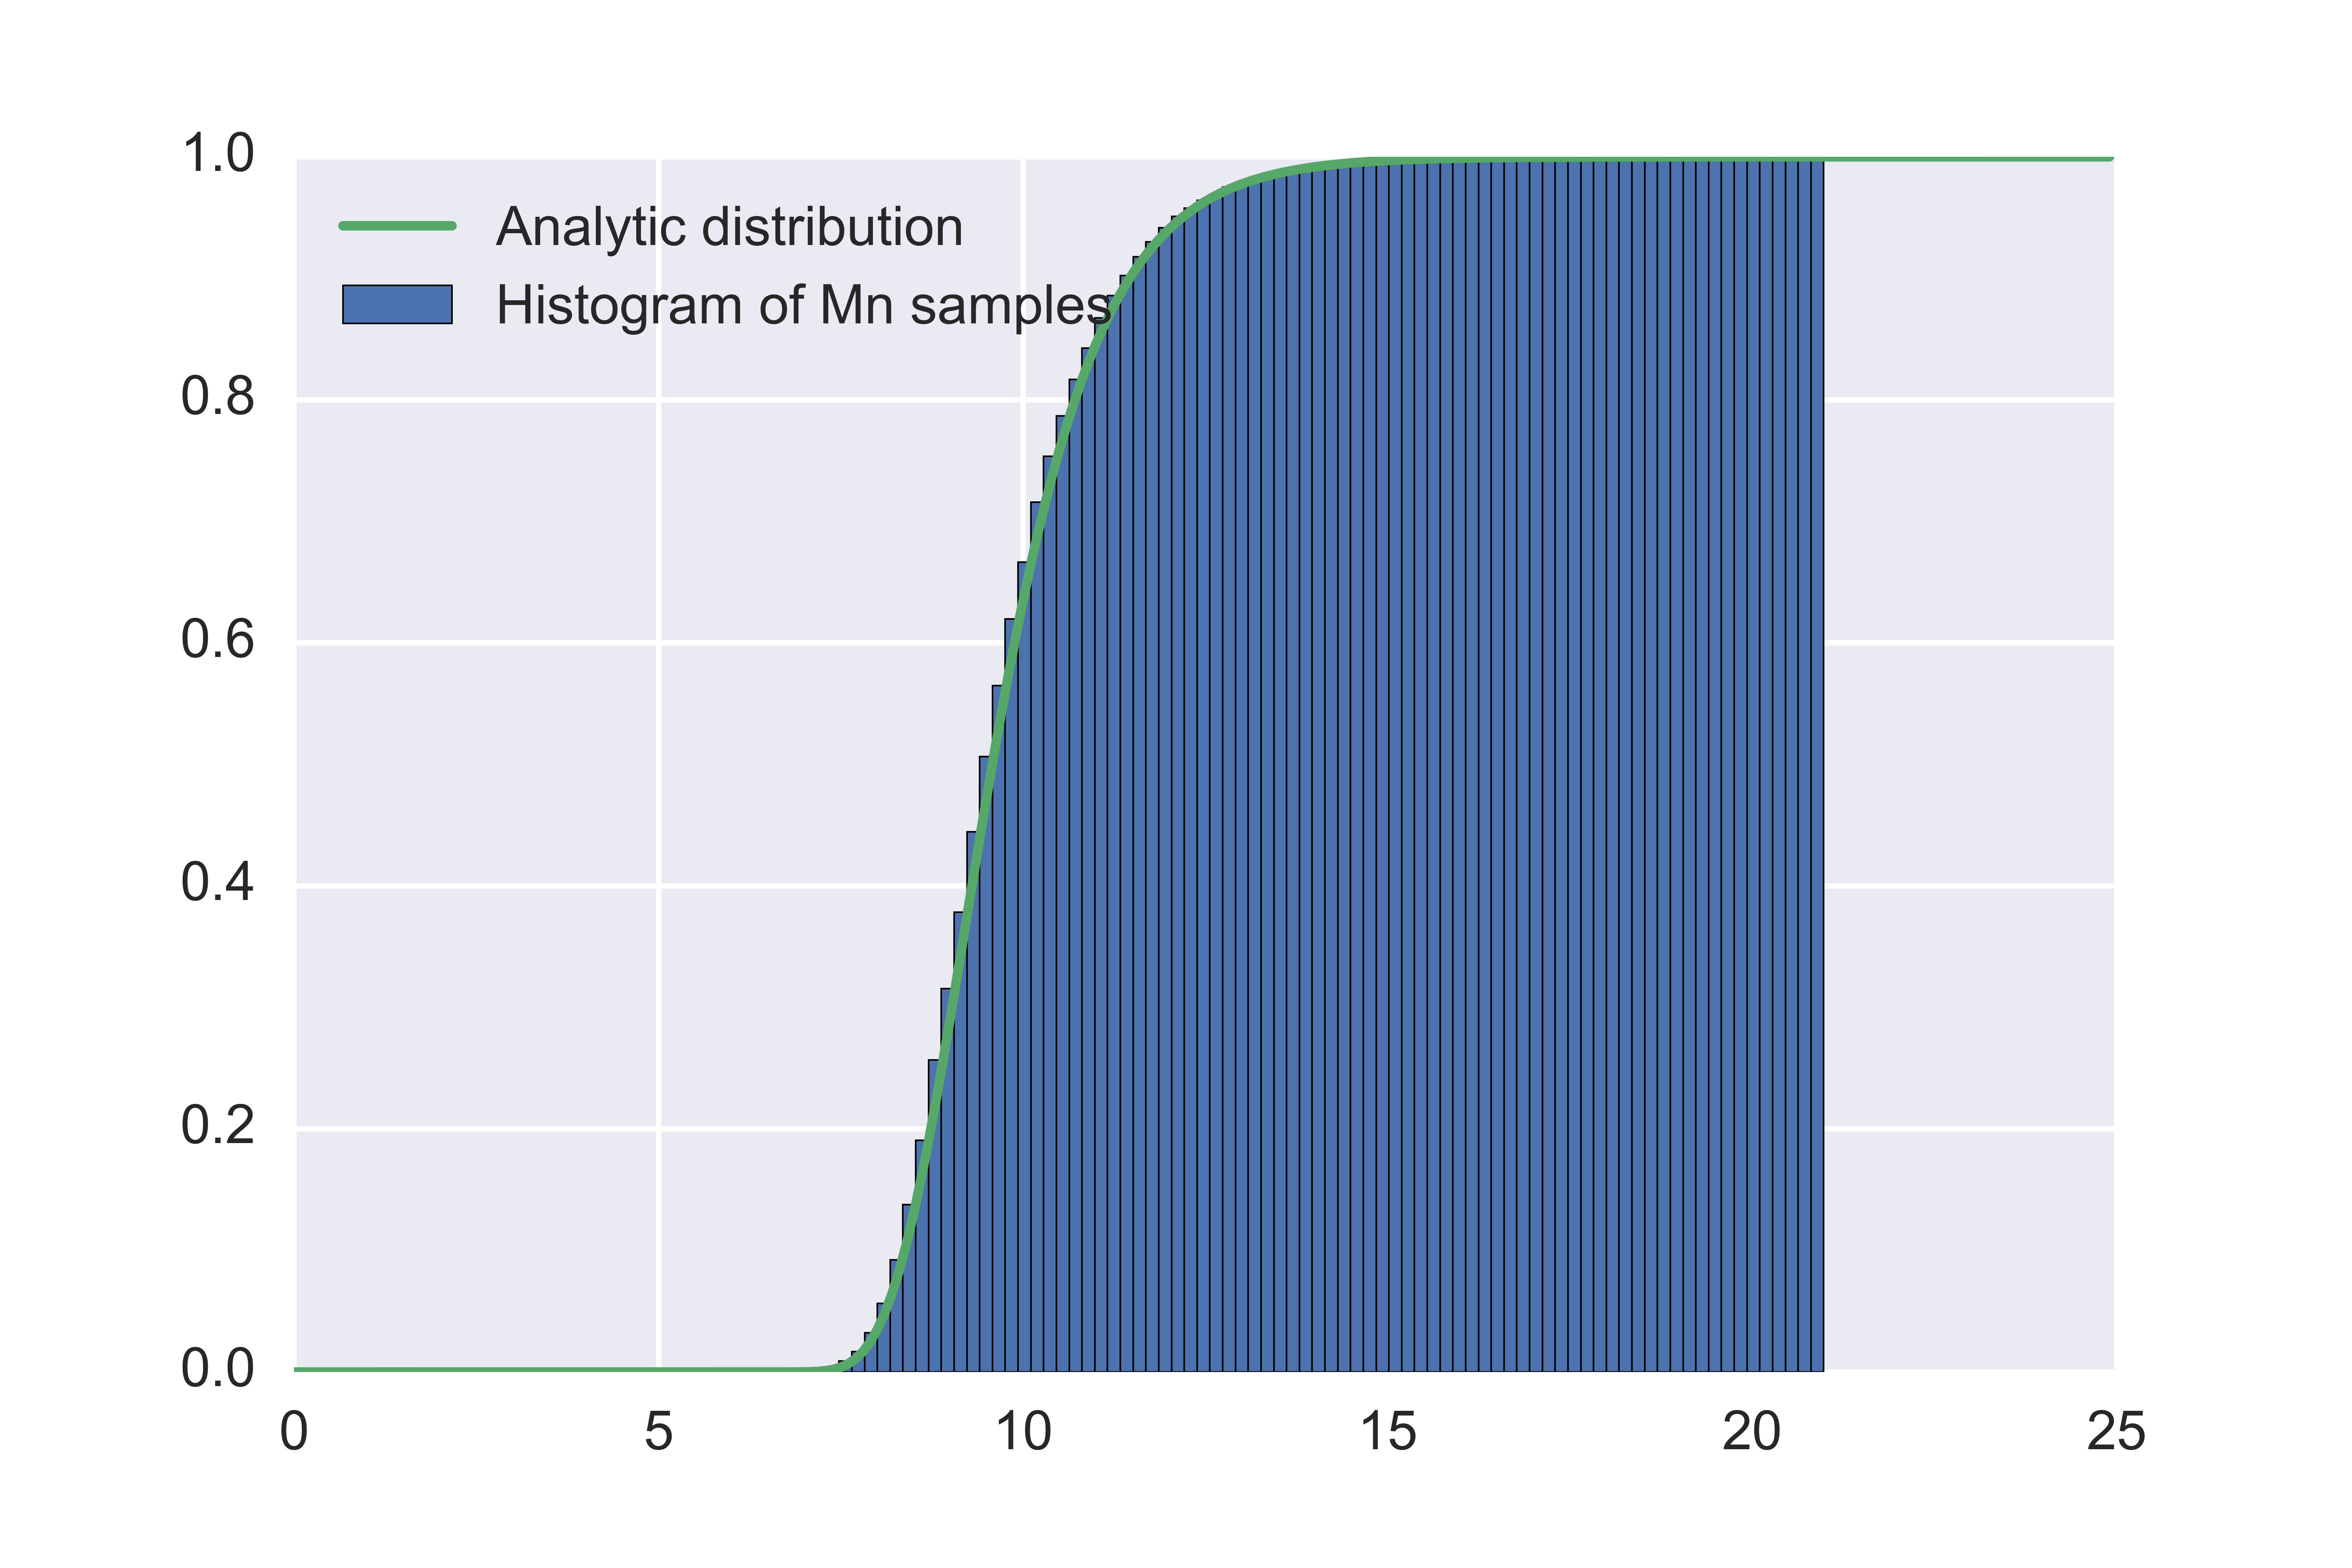
\includegraphics[scale=0.75]{example1.png}
\end{figure}
\end{frame}
\end{document}

